\documentclass[tikz,border=3pt]{standalone}
\usepackage{pgfplots}
\pgfplotsset{compat=1.18}
\begin{document}
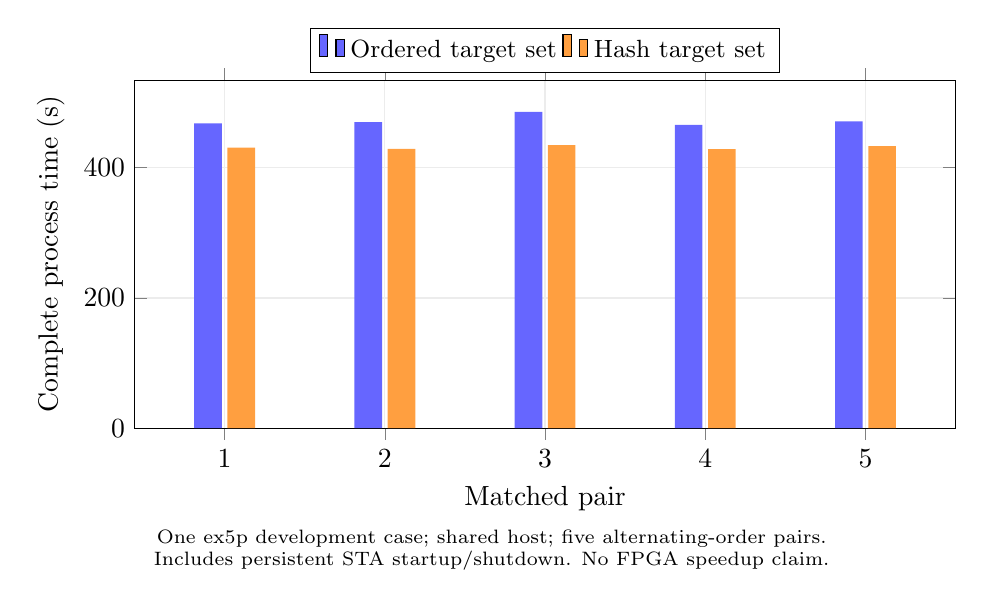
\begin{tikzpicture}
\begin{axis}[width=12cm,height=6cm,ybar,bar width=10pt,ymin=0,xlabel={Matched pair},ylabel={Complete process time (s)},xtick={1,2,3,4,5},enlarge x limits=.14,grid=major,grid style={gray!15},legend style={at={(.5,1.02)},anchor=south,legend columns=2,font=\small}]
\addplot[fill=blue!60,draw=none] coordinates {(1,468.170780456) (2,470.086914457) (3,485.901425867) (4,466.035399696) (5,471.36454189)};
\addplot[fill=orange!75,draw=none] coordinates {(1,431.071811383) (2,429.051663084) (3,434.729429842) (4,428.54164886) (5,433.399655937)};
\legend{Ordered target set,Hash target set}
\end{axis}
\node[anchor=north,font=\scriptsize,align=center] at (current bounding box.south) {One ex5p development case; shared host; five alternating-order pairs.\\Includes persistent STA startup/shutdown. No FPGA speedup claim.};
\end{tikzpicture}
\end{document}
